\section{Implementation}
Our prototype implementation of \system{} is based on a series of relays, an oracle, and 
a client. All \system{} software can be found at ... \annie{I'll add in wherever we end 
putting it anonymously}

{\bf Relays.}  We established nine relays, one in each of the following countries: Brazil, 
Germany, Singapore, Japan, Australia, France, United States, United Kingdom, and Canada; these 
are shown, along with their corresponding AS number in Figure \ref{fig:relay_locations}.  
They are running as Ubuntu Virtual Private Servers (VPSs) with 
Squid as the proxy server.  They are also running the \system{} Relay software.

\begin{figure}[b!]
\centering
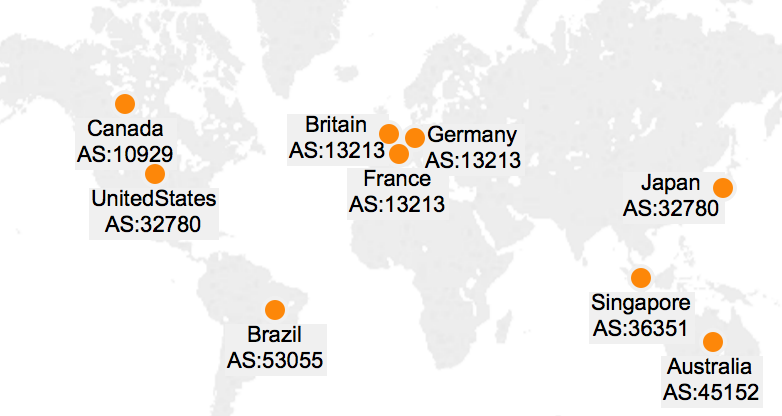
\includegraphics[width=.5\textwidth]{relay_map}
\caption{The locations and ASNs for \system{} relays.}
\label{fig:relay_locations}
\end{figure}

{\bf Oracle.}  The oracle is a Fujitsu RX200 S8 server with dual, 
eight-core 2.8GHz Intel Xeon E5 2680 v2 processors with 256GB RAM running the 
Springdale distribution of Linux. It is running the \system{} Oracle software, 
which interacts with relays and with RIPE Atlas probes.

{\bf Client.} For the purposes of the system evaluation, we set up a client 
machine in the Netherlands, which simply accesses web content and uses the PAC 
file generated by the oracle. 
